\chapter{Design and Implementation}\label{implement}

    In this chapter, the implementation details will be explained in many aspects, including Java Native Interface,
    human detection, and distance calculation.

    \section{Preparation}
        This application is implemented on the Android Operating System,
        and the target Software Development Kit (SDK) version is set at level 29, namely Android Q.
        This application is compiled and built by Android Studio version 3.5.3,
        and CMake is used for compiling C++ library with C++ version 11.
        Furthermore, OpenCV version 4.4.0, which is built as shared library, is used for image processing and object detection.
        For object detection model, there are 2 models are used: You Only Look Once and MobileNet SSD.

    \section{Java Native Interface}
        Implementation is divided into 3 layers.
            The first layer is a Java layer, which mainly interacts with a user,
            checks permissions, handles activity lifecycle, communicates with Java Native Interface (JNI), and loads native libraries.
                native libraries are compiled and built into shared libraries by a Native Development Kit (NDK).
            The second layer is JNI, which is written in C or C++.
                The task of JNI layer is being an intermediate connection between the Java layer and a C++ layer.
            The last layer is the C++ layer, which alternatively performs calculation tasks,
            including Deep Neural Network and distance calculation.

        \begin{figure}[!ht]
            \centering
            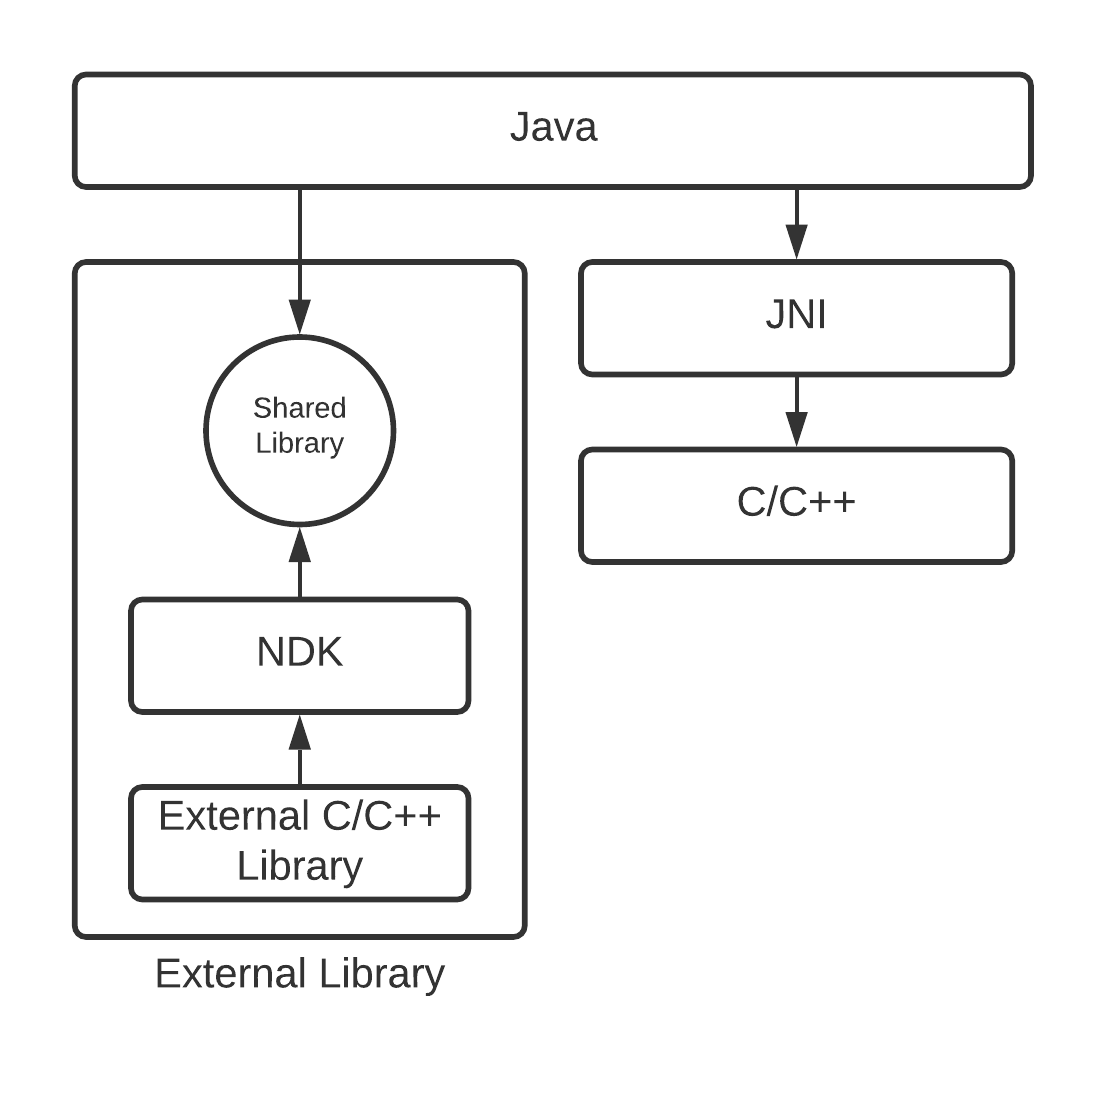
\includegraphics[width=4in]{images/chapter3/application-layers.png}
            \caption{Application Layers}
            \label{systemOverview}
        \end{figure}

        However, Deep Neural Network and distance calculation can be implemented in all layers.
        According to Android Developer Guide \cite{ANDROID-01},
        Native Development Kit (NDK) is recommended for compiling C and C++ coode into native library,
        which is able to achieve a higher performance.
        Thus, executing both tasks in the JNI and C++ layer gains a better performance.
        Furthermore, there are 2 advantages of implementing JNI.
            The first advantage is reducing JNI calling. Performing both tasks in an application layer have to call JNI methods many times,
                and this is expensive and cost an overhead.
                Thus, implementing JNI manually reduces the number of JNI calls.
            The second advantage is memory management. C++ is able to access values in the memory by using a pointer.
                Thus, values can be directly accessed without copying.

        Java and JNI communicate through native function, which is written in Java layer.
        Memory addresses of pre-processed frame in Mat format will be pass as parameter through native function,
        and it will be converted from Java type to Native type.
        Then, the given addresses will be converted back into Mat format.

\begin{lstlisting}[caption={Java Native Function},captionpos=b]
    public class NativeLib {
        static {
            System.loadLibrary("native-lib");
        }

        public native static void process(long imageAddr);
    }
\end{lstlisting}

\begin{lstlisting}[caption={C++ JNI Method},captionpos=b]
    Java_com_jinkawin_dissertation_NativeLib_process(jlong matAddr){
        Mat &frame = *(Mat *) matAddr;
        ImageProcessor::process(frame);
    }
\end{lstlisting}

    \section{Social Distancing Detection}
        % Intro to detection
        There are 3 main processes is implemented to determine social distancing violation from the image and video.

        The first process is pre-processing the given image, video, or video stram.
        The given video will be extracted into an array of images.
        Then, images will be converted into Bitmap and Mat format with RGBA colour model respectively.
        After that, colour will be converted, which depends on a detection model.
        As mentioned in section 4.1, there are 2 detection models are used for detecting humans in the given picture and video: YOLO model and MobileNet SSD model.
        Colour will be converted to RGB if the detection model is YOLO,
        while MobileNet SSD requires BGR colour model.

        \begin{figure}[!ht]
            \centering
            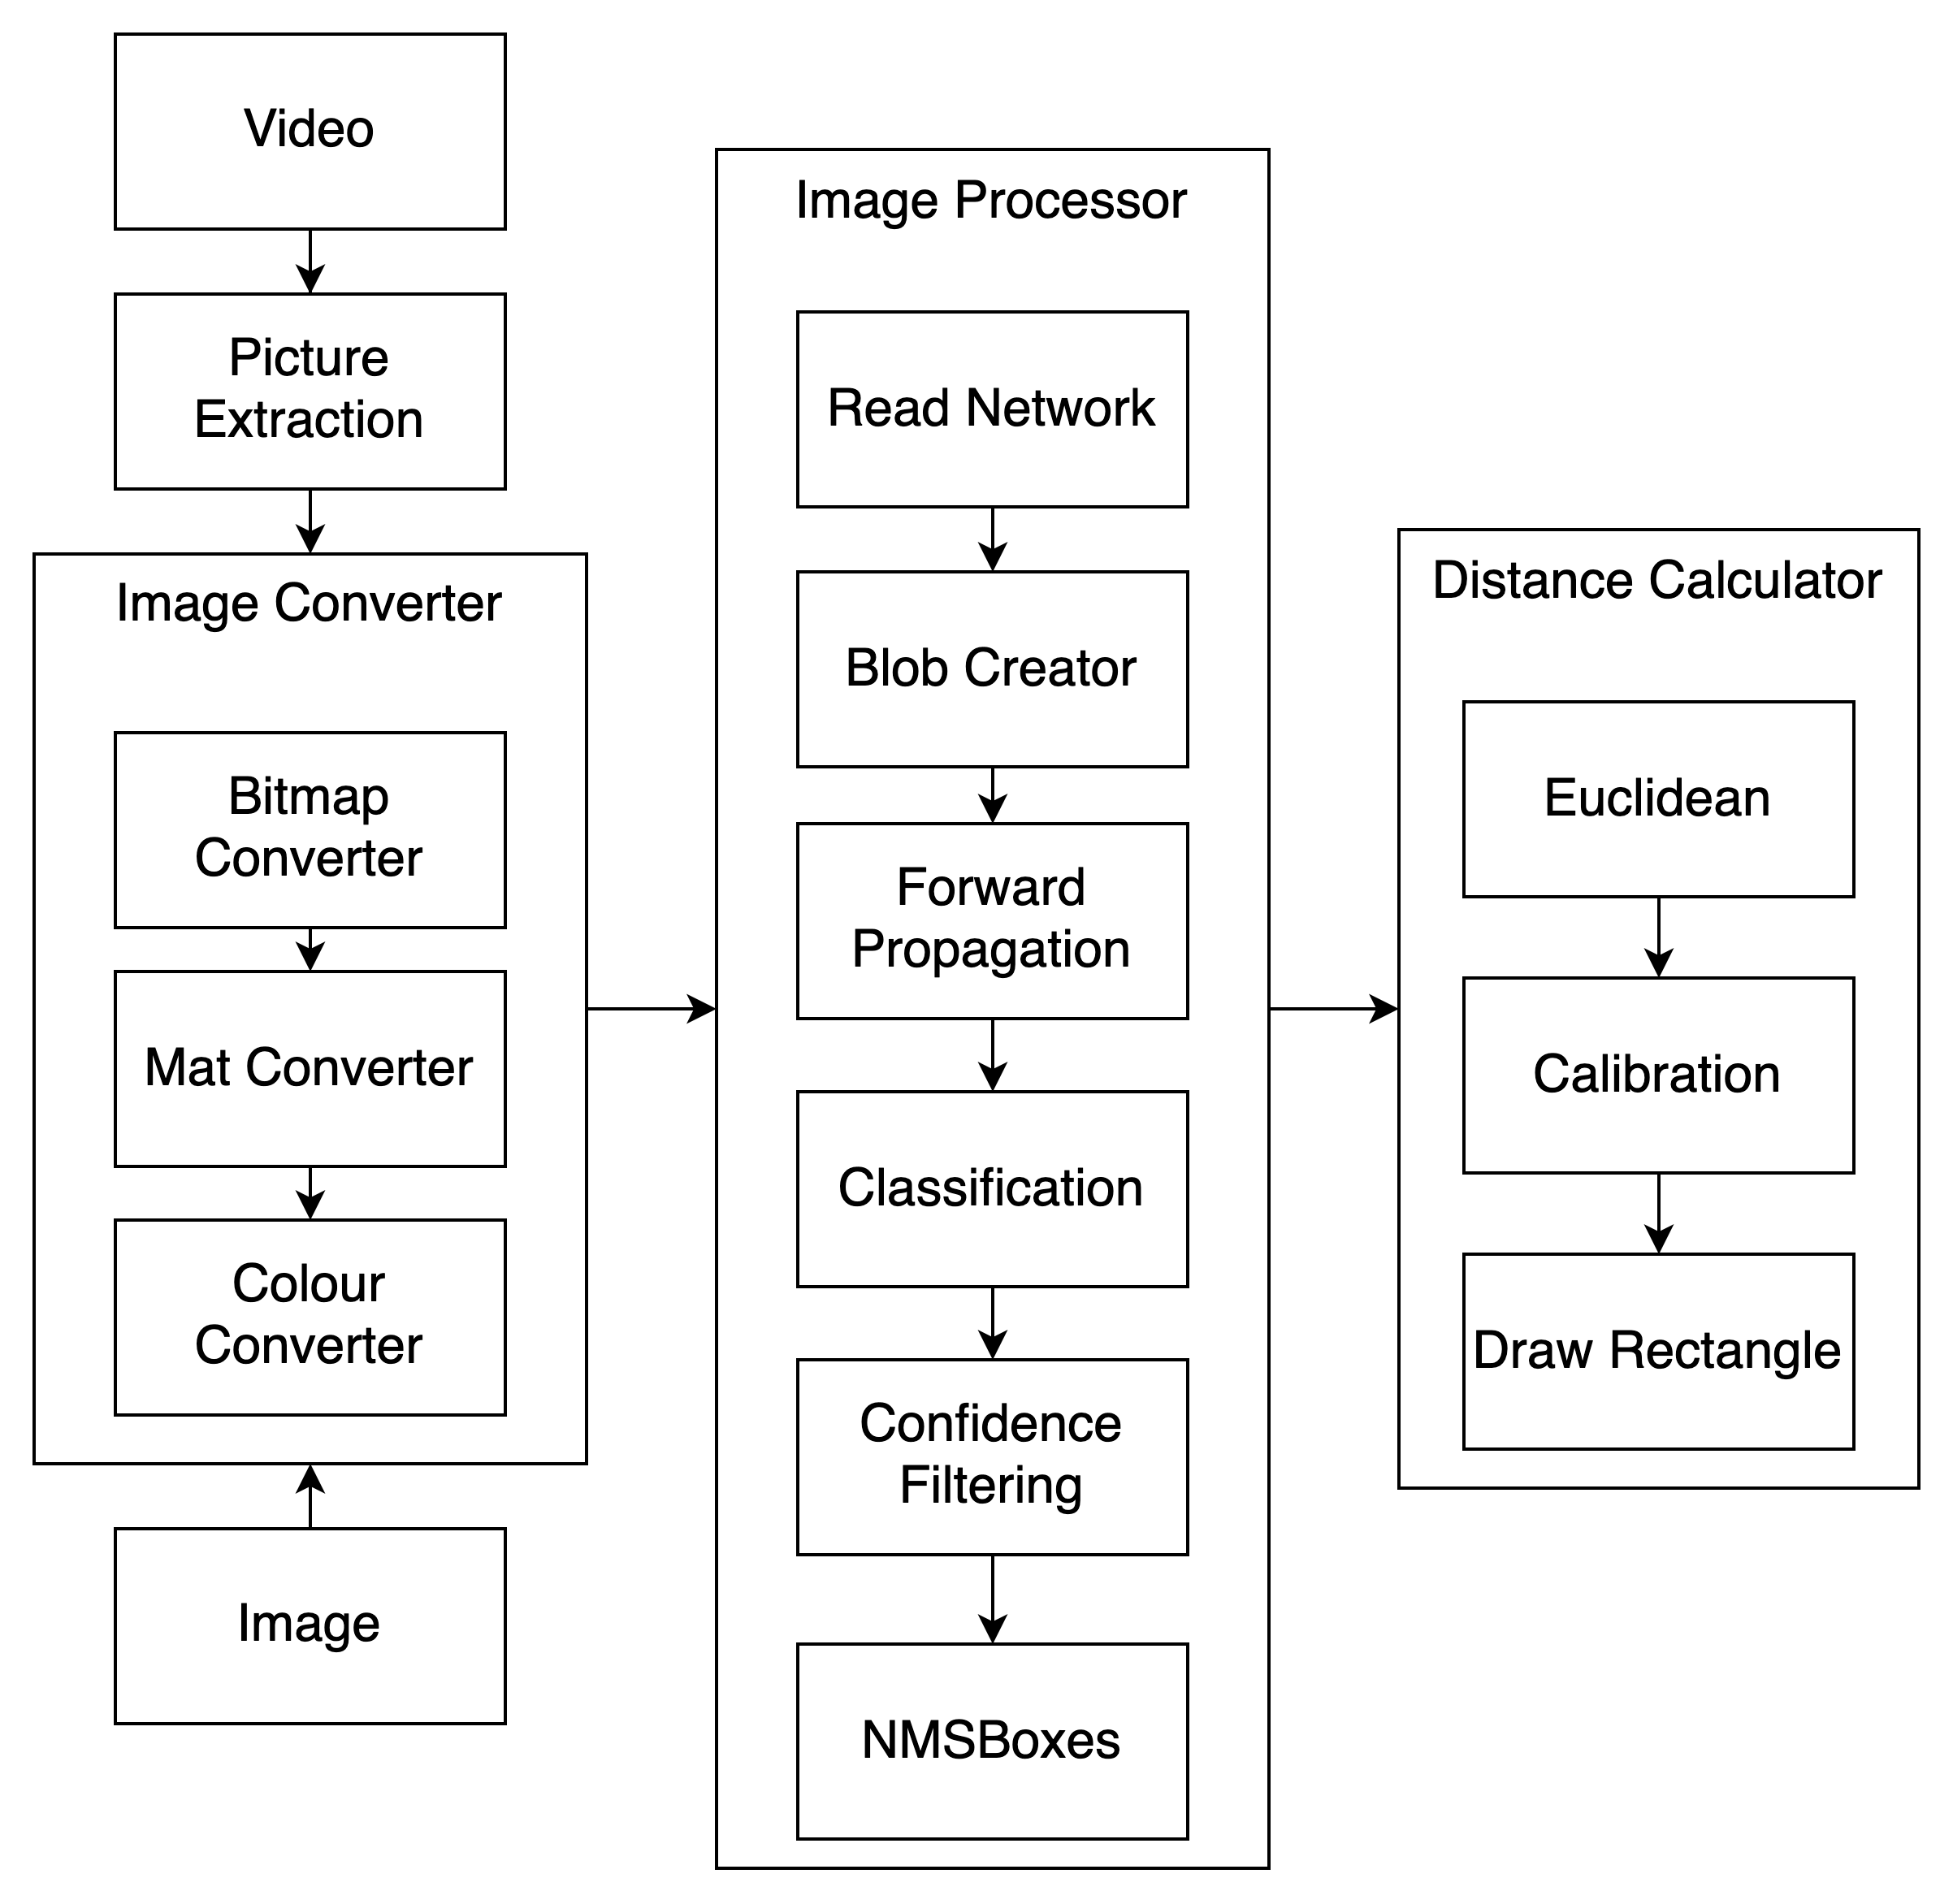
\includegraphics[width=5in]{images/chapter3/system-overview.png}
            \caption{Detection System Overview}
            \label{systemOverview}
        \end{figure}

        The second process is object detection.
        Detection models are setup and configured differently before processing images.
        First of all, YOLO is used with Darknet, which is an open source neural network framework,
            while MobileNet SSD. MobileNet is used with Caffe framework.
        Then, threshold will be set for determining the confidence level of the detected object.
            The confidence level threshold of YOLO model will be set to 0.5 or 50 percent.
            In other words, the detected object will be rejected if YOLO model cannot guarantee that a detected object is human,
            and its confidence level is lower than 50 percent.
            In contrast, The confidence level threshold of MobileNet SSD model will be set to 0.3 or 30 percent.
            Because of MobileNet SSD model has a lower ability to detect an object, the confidence threshold is set to be lower.
        After models are setup and configured, the image will be processed in 5 steps.
        For the first step, pre-processed image will be convert to input blob by passing Mat image to $blobFromImage()$ function with scale factor.
            Blob will be used for the forward propagation in the neural network.
        Secondly, blob will be passed to the network through $forward()$ function,
            and the network's output is a list of detected boxes with a label and a confidence level.
        Then, detected objects will be classified.
            Non-human objects will be removed by considering the label of the detected object.
        After that, a confidence level will be filtered by considering the threshold that is set in the configuration step.
        Finally, $NMSBoxes()$ performs non-maximum suppression, which will reduce overlapping detected boxes.

        The last process is determining social distancing.
        After a list of detected object boxes is filtered,
        the distance between each box will be calculated by using the formula which is based on Euclidean distance
        \footnote{an explanation was given in chapter \ref{background}}.
        If the value of the calculated distance is lower than the threshold,
        this mean that the couple is too close, and they are breaking social distancing rule.
        The application will change the box's colour to red.
        In contrast, if the value of the calculation is grater than threshold,
        there is no breaching of social distancing rule, and the box's colour will be changed to green.

    \section{Parallelisation}
        Multithreading is used to reduce the processing time, which can achieve nearly real-time processing.
        The strategy of multithreading is dividing an input video into frames,
        and assign frames to threads by considering a number of available cores.

        \subsection{Multitheading with Java}

            To begin with, a processor manager is implemented for managing threads efficiently.
            To ensure that the processor manager will be created at once,
            the processor manager is designed with singleton pattern and static block.
            Thread pool and queues are fundamental operators in the processor manager.
            As can be seen in figure \ref{parallelJava}, frames in Mat format will be assigned as a task and queued in TaskQueue.
            Then, tasks will be mapped with thread orderly by the thread pool.
            A working thread will process the given task.
            After a thread finished the given task,
            the thread will write a log regarding social distancing detection, and notify the processor manager.
            Then, a task will be recyled to free up memory.
            When the processor manager receive a notification from workers,
            a processed frame will be retrieved and ordered in the priority queue.
            After the process manager retrieved all processed frames,
            the process manager will notify the main activity.
            All of these processes are run in the background to avoid a frozen application.

            \begin{figure}[!ht]
                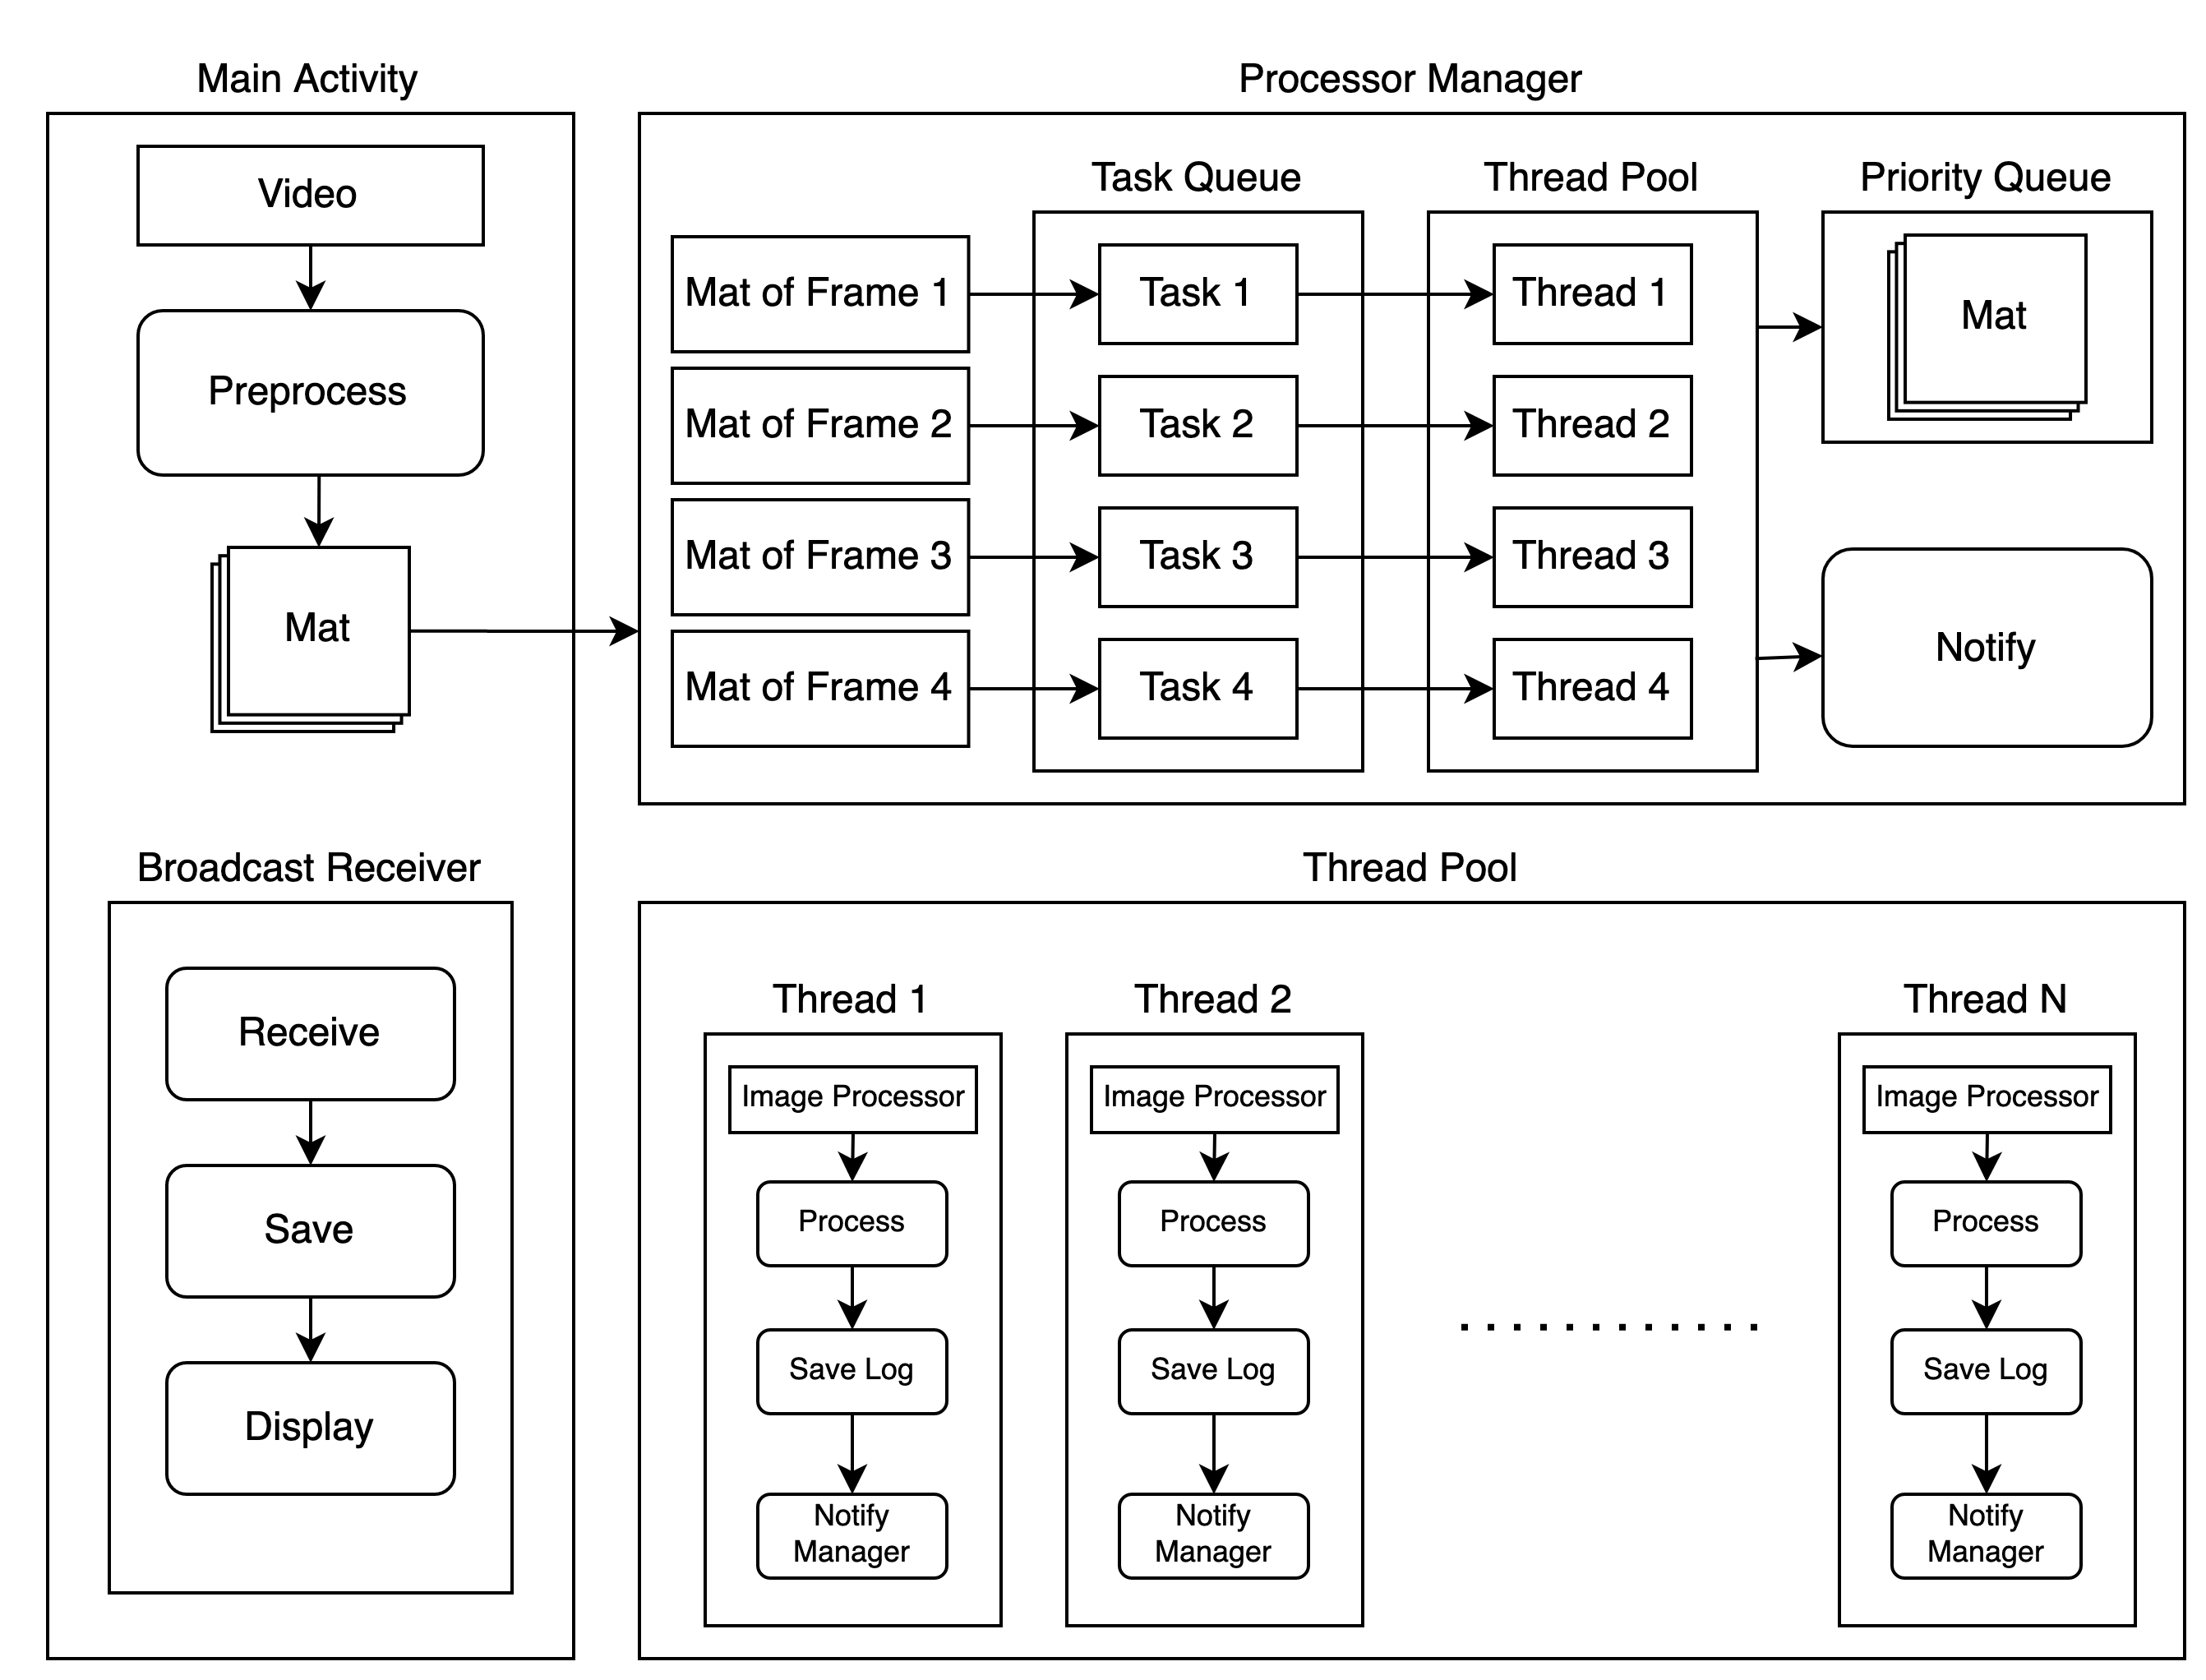
\includegraphics[width=6in]{images/chapter3/parallel.png}
                \caption{Parallel Computing Diagram}
                \label{parallelJava}
            \end{figure}

        \subsection{Multitheading with C++}

\begin{lstlisting}
    virtual void operator()(const cv::Range& range) const{
        for (size_t i = range.start; i < size; i += threadNo){
            cv::Mat &frame = *(cv::Mat *) frames[i];
            ImageProcessor::process(frame);
        }
    }
\end{lstlisting}

        - How to show processed frame from live stream?
